\documentclass[12pt]{article}

% refer to configurations.tex for the LaTeX setup of this template
\usepackage[english]{babel}
\usepackage{pythonhighlight}
\usepackage{graphicx}
\usepackage{minted}
\usepackage{setspace}

\title{\textbf{\textsf{Exploring Cellular Automata}}}
\date{\today}
\author{}
% math
\usepackage{amsmath, amssymb}

% references
\usepackage[style=apa, backend=biber]{biblatex}
\addbibresource{bibliography.bib}

% Increase spacing between bibliography entries
\setlength{\bibitemsep}{1em} % Adjust spacing between bibliography entries
\setlength{\bibhang}{2em}    % Adjust hanging indentation

% fonts
\usepackage{helvet}
\usepackage{sectsty}
\allsectionsfont{\sffamily} % for section titltes use sans-serif
% \renewcommand{\familydefault}{\sfdefault} % comment out for sans-serif font
% \usepackage{sansmath} % comment out for sans-serif math font
% \sansmath % comment out for sans-serif math font

% margins
\usepackage{geometry}
\geometry{
  a4paper,
  total={170mm,257mm},
  left=25mm,
  right=25mm,
  top=30mm,
  bottom=30mm,
}

% no indentation when a new paragraph starts
\setlength{\parindent}{0cm}

% links
\usepackage{hyperref} % better links
\usepackage{color}    % nicer link colors
\definecolor{pigment}{rgb}{0.2, 0.2, 0.6}
\hypersetup{
  colorlinks = true, % Color links instead of ugly boxes
  urlcolor   = pigment, % Color for external hyperlinks
  linkcolor  = black, % Color for internal links
  citecolor  = pigment % Color for citations
}

% headers
\usepackage{fancyhdr}
\pagestyle{fancy}
\lhead{Developing a engine to simulate cellular automata and analyze their evolution.}
\chead{}
\rhead{}

% example boxes
\usepackage{tcolorbox}
\newtcolorbox{examplebox}{
  colback=white,
  colframe=gray!30,
  title=Example,
  sharp corners,
  boxrule=0.5pt,
  coltitle=black
}

% conditionals
\usepackage{ifthen}
\newboolean{showinstructions}
\newboolean{showexamples}
\newboolean{showexplanations}
\renewenvironment{examplebox}{%
  \ifthenelse{\boolean{showexamples}}%
    {\begin{tcolorbox}[colback=white, colframe=gray!30, title=Example, sharp corners, boxrule=0.5pt, coltitle=black]}%
    {\expandafter\comment}%
}{%
  \ifthenelse{\boolean{showexamples}}%
    {\end{tcolorbox}}%
    {\expandafter\endcomment}%
}

% Define a new environment for explanations
\newcommand{\explanation}[1]{%
  \ifthenelse{\boolean{showexplanations}}%
    {\textit{Explanation:} #1}%
    {\ignorespaces}%
}

% Define a new environment for instructions
\newcommand{\instructions}[1]{%
  \ifthenelse{\boolean{showinstructions}}%
    {#1}%
    {\ignorespaces}%
}

\makeatletter
\newcommand{\maketitlepage}{%
    \begin{titlepage}
        \maketitle
        \thispagestyle{empty}
        \vfill 
        \centering
        Abrar Habib \\
        CSc 59866 - Senior Project I \\
        The City College of New York \\
        % Template based on the paper: \\
        
        \vfill 
    \end{titlepage}
    \newpage
}
\makeatother


\setlength{\parindent}{20pt} % Indent size
\setlength{\parskip}{0em}    % Space between paragraphs

% Optional user settings
\setboolean{showinstructions}{true} % set to false to hide instructions
\setboolean{showexamples}{true} % set to false to hide examples
\setboolean{showexplanations}{true} % set to false to hide explanations

\begin{document}
\maketitlepage
\tableofcontents
\newpage
\doublespacing

\instructions{\section{Introduction}
	\subsection{Overview}
	Cellular automata (CA) are computational models used to simulate complex
	systems through simple, discrete rules applied across a grid of cells.
	Each cell in the grid updates its state based on a fixed set of rules
	that consider the states of neighboring cells. Despite their simplicity,
	cellular automata can exhibit rich, emergent behavior, making them powerful
	tools for studying dynamical systems, pattern formation, and decentralized
	computation. From modeling physical phenomena like fluid dynamics and crystal growth to simulating ecosystems and traffic flow, CA offer a flexible framework for exploring how local interactions give rise to global behaviors.

	This project focuses on developing a simulation tool for cellular automata, with the initial goal of implementing Conway's Game of Life, a well-known CA that demonstrates how simple rules can produce complex and often unpredictable patterns. The project aims to provide a robust and extensible platform for exploring a variety of rule sets, enabling users to experiment with different configurations and observe the resulting dynamics. By allowing custom rules and initial states, the simulation supports creative exploration and deepens understanding of how individual components interact over time.

	Beyond recreational use and theoretical exploration, cellular automata have practical applications in computer science, biology, and physics. They have been used in parallel computing models, procedural content generation, and even in modeling biological processes such as cell differentiation and tissue growth. As digital systems generate increasing volumes of data and demand efficient modeling approaches, CA remain relevant as intuitive yet powerful tools for simulating complexity. This project leverages that potential, offering both an educational platform and a stepping stone for further applications in research and development.

	\subsection{Motivation}

	The motivation behind this project was driven by curiosity, simplicity, and fun. After encountering cellular automata in class, I was intrigued by how such simple rules could produce such complex, emergent behavior. It seemed like a project I could build relatively quickly while still offering plenty of room for deeper exploration. The idea of simulating life-like behavior through deterministic logic was both intellectually satisfying and creatively engaging.

	What really pushed me to start the project was a video I came across, which showed how Conway’s Game of Life could be used to simulate itself. That demonstration, built on the fact that the Game of Life is Turing complete, blew my mind. While I didn’t reach that level of complexity in my own implementation, the process gave me a much deeper understanding of how cellular automata operate and how small rule changes can lead to drastically different behaviors.

	This project also gave me a great opportunity to write clean and modular code in Rust. Exploring cellular automata became more than just a quick project—it became a fun and rewarding deep dive into simulation, emergent systems, and creative problem solving.
}

\section{Tech Stack}
\subsection{Rust}
The entire project is written in Rust. I didn't really use any third party libraries except two: Clap and Ratatui. Clap is a library that makes it extremely easy to set up a command line interface for my project. I just created a struct called Cli and then I use a match statement to handle the different arguments the user provides. The second library I used was ratatui, which helps in interfacing with a terminal (usually for drawing things or UI's).

The CA itself was just represented by a struct with fields for it's size, the rule, and general data. To simulate the automaton, I just use a for loop alongside the rule provided to create a new grid of the next "tick" of simulation. At each tick, the current grid is converted to a string with special unicode characters to represent a live cell and then passed to ratatui to be displayed on the terminal screen.

\subsection{Python}
To generate the graphs that I displayed during the presentation, I used a simple Python script using matplotlib and pandas. In the Rust code, each automaton keeps track of its entropy and cell count over time. After the simulation is terminated, the program writes all the stats to a csv file. I made a little bash script to automatically run the two different programs (the Rust program to run the simulation and the Python program to plot the graph). The Python script will read the csv file generated, plot the results, and then display it for me to view, save, edit, or do whatever I want with it.

\subsection{Source Code}
Here is the struct that represents the automaton. It contains the width and height of the grid, a vector of cells, the rule, and some other stats like generation count and live cell count.
\begin{singlespace}
	\begin{minted}[fontsize=\small]{rust}
// Conway's Game of Life rule implementation in Rust
pub struct Automaton {
    pub width: usize,    // Number of columns in the grid
    pub height: usize,   // Number of rows in the grid
    pub grid: Vec<Cell>, // 1D flattened representation of the 2D grid
    pub rule: Rule,      // Birth/survival rules that define cell behavior
    pub generation: usize,
    pub live_cells: usize,
}
\end{minted}
\end{singlespace}
We can also define some methods on an automaton to help drive the simulation.

\begin{singlespace}

	\begin{minted}{rust}
impl Automaton {
    pub fn new(width: usize, height: usize, rule: Rule) -> Self {
        Self {
            width,
            height,
            grid: vec![Cell::Dead; width * height],
            rule,
            generation: 0,
            live_cells: 0,
        }
    }

    pub fn tick(&mut self) {
        let mut new_grid = self.grid.clone();
        let mut next_live_count = 0;

        for y in 0..self.height {
            for x in 0..self.width {
                let idx = self.index(x, y);
                let live_count = self.live_neighbor_count(x, y);
                let cell = self.grid[idx];

                new_grid[idx] = match cell {
                    Cell::Alive => {
                        if self.rule.survive.contains(&live_count) {
                            next_live_count += 1;
                            Cell::Alive
                        } else {
                            Cell::Dead
                        }
                    }
                    Cell::Dead => {
                        if self.rule.birth.contains(&live_count) {
                            next_live_count += 1;
                            Cell::Alive
                        } else {
                            Cell::Dead
                        }
                    }
                }
            }
        }

        self.grid = new_grid;
        self.generation += 1;
        self.live_cells = next_live_count;
    }

    pub fn set_alive(&mut self, x: usize, y: usize) {
        if x < self.width && y < self.height {
            let idx = self.index(x, y);
            self.grid[idx] = Cell::Alive;
        }
    }

    pub fn as_string(&self) -> String {
        let mut output = String::new();
        for y in 0..self.height {
            for x in 0..self.width {
                let cell = self.grid[self.index(x, y)];
                output.push(if cell == Cell::Alive { '#' } else { ' ' });
            }

            output.push('\n');
        }
        output
    }

    fn live_neighbor_count(&self, x: usize, y: usize) -> u8 {
        let mut count = 0;
        let width = self.width as isize;
        let height = self.height as isize;

        for dy in [-1, 0, 1] {
            for dx in [-1, 0, 1] {
                if dx == 0 && dy == 0 {
                    continue;
                }

                let nx = (x as isize + dx + width) % width;
                let ny = (y as isize + dy + height) % height;

                let idx = self.index(nx as usize, ny as usize);
                if self.grid[idx] == Cell::Alive {
                    count += 1;
                }
            }
        }

        count
    }
}
\end{minted}

\end{singlespace}
While the syntax is a bit different, it still is readable and should clearly convey how
I implemented certain features. I also wanted to demonstrate how rules are applied to a simulation.
The Rule struct has two vectors that represent the number of neighbors that need to be alive
for the cell to be born and keep surviving.
\begin{singlespace}

	\begin{minted}[fontsize=\small]{rust}
    #[derive(Debug, Clone)]
    pub struct Rule {
        pub birth: Vec<u8>,
        pub survive: Vec<u8>,
    }
    
    impl Rule {
    pub fn from_str(rule_str: &str) -> Result<Self, RuleError> {
        let parts: Vec<&str> = rule_str.trim().split("/").collect();

        if parts.len() != 2 {
            return Err(RuleError::InvalidFormat);
        }

        let birth_str = parts[0].strip_prefix("B").ok_or(RuleError::MissingPrefix)?;
        let survive_str = parts[1].strip_prefix("S").ok_or(RuleError::MissingPrefix)?;

        let birth: Result<Vec<u8>, RuleError> = birth_str
            .chars()
            .map(|c| {
                c.to_digit(10)
                    .map(|n| n as u8)
                    .ok_or(RuleError::InvalidDigit(c))
            })
            .collect();

        let survive: Result<Vec<u8>, RuleError> = survive_str
        .chars()
        .map(|c| {
            c.to_digit(10)
                .map(|n| n as u8)
                .ok_or(RuleError::InvalidDigit(c))
        })
        .collect();

        Ok(Self {
            birth: birth?,
            survive: survive?,
        })
    }
}
\end{minted}
\end{singlespace}

\section{Results}

\subsection{Initial Results}
This isn't necessarily a project where you can measure it's results. I mean, what does it even mean to measure the results of what is effectively a library? Instead, I will be showing graphs and other data from a few runs of the simulation based on different rules.

The first graph I want to show is from a run where the rule was Conway's Game of Life.
Since the simulation keeps track of the live cell count and entropy of the grid, we can graph those two metrics.

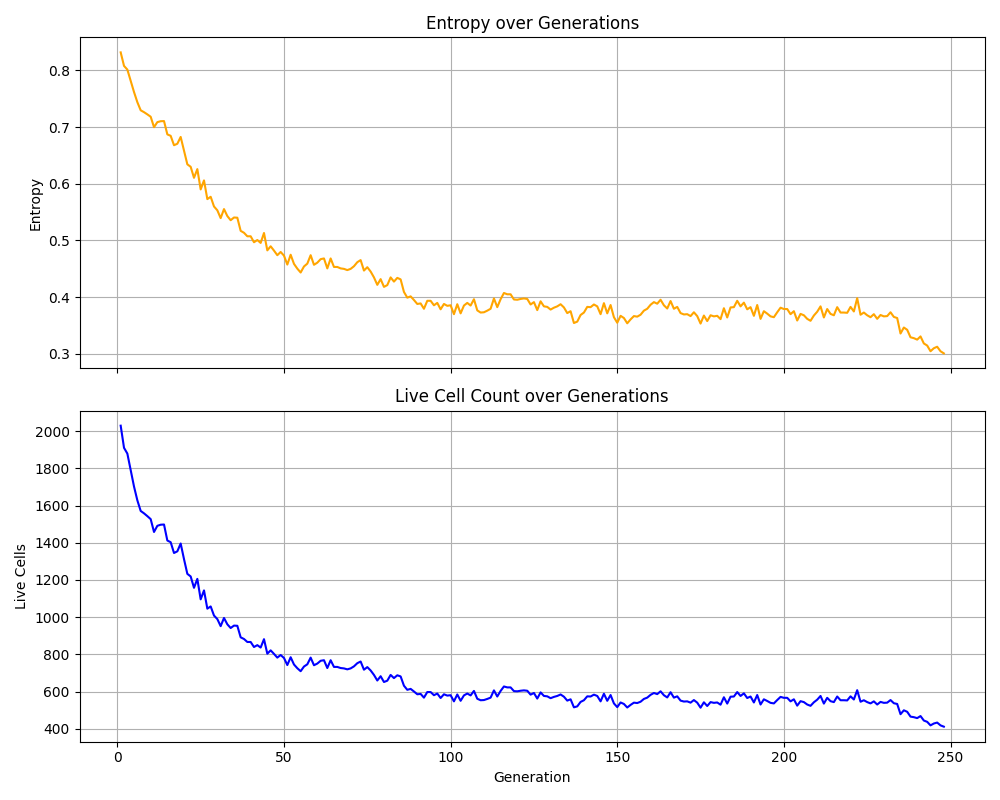
\includegraphics[scale=0.6]{../figures/Figure_1.png}

We begin the simulation with a random grid of alive and dead cells, which is shown by the high entropy and high population count. As time moves on however, we start to get a lower state of entropy and also a lower cell count. This shows that the rules for Conway's Game of Life enables the system to self organize from chaos into partially stable and localized structures. Similarly, the evolution of the cell counts show that the game rapidly prunes unstable or overpopulated regions, then converges to a dynamic equillibrium of still ifes and oscillators, with gliders dying over time.

The second graph is from a rule called Diamoeba. This rule is meant to produce amoeba-like structures that move and grow like actual amoebas.

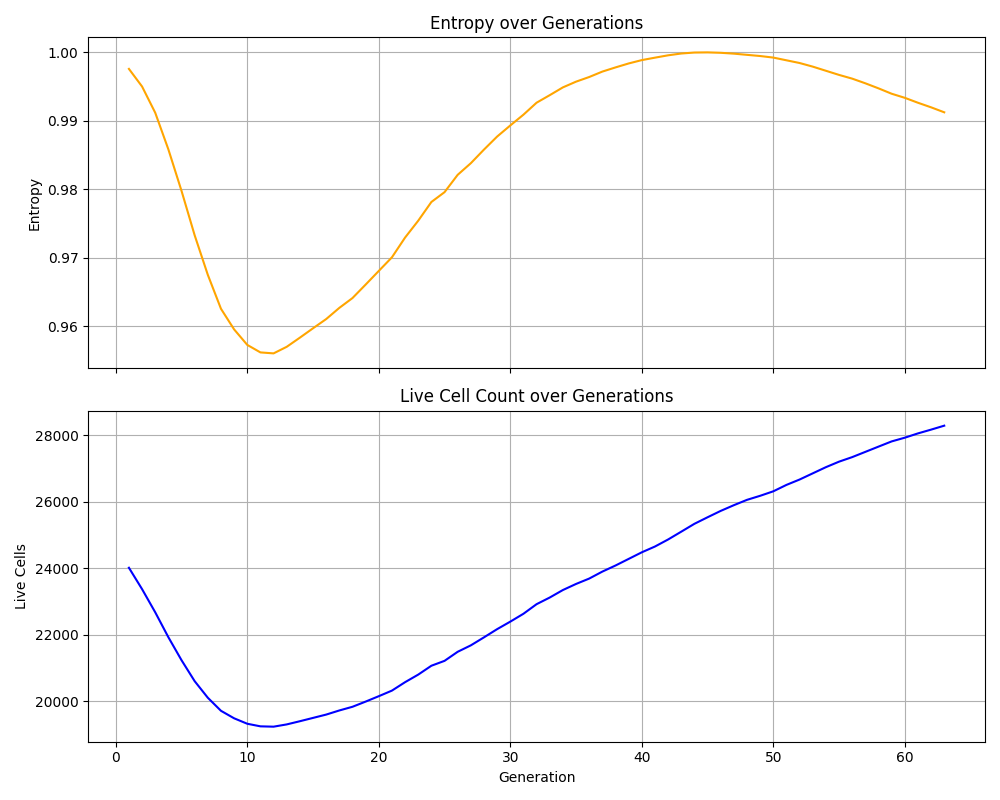
\includegraphics[scale=0.6]{../figures/Figure_2.png}

Once again, we start off with high entropy, which makes sense since we have a random state of cells at the beginning. After some ticks, we start generating individual clusters that then grow for the remainder of the program until the entire grid is just full of alive cells. Similarly, with the cell count, the game prunes unstable and overpopulated regions. Certain regions that managed to stay alive start clustering and growing.

Lastly, is the graph from a rule for a maze-like structure.

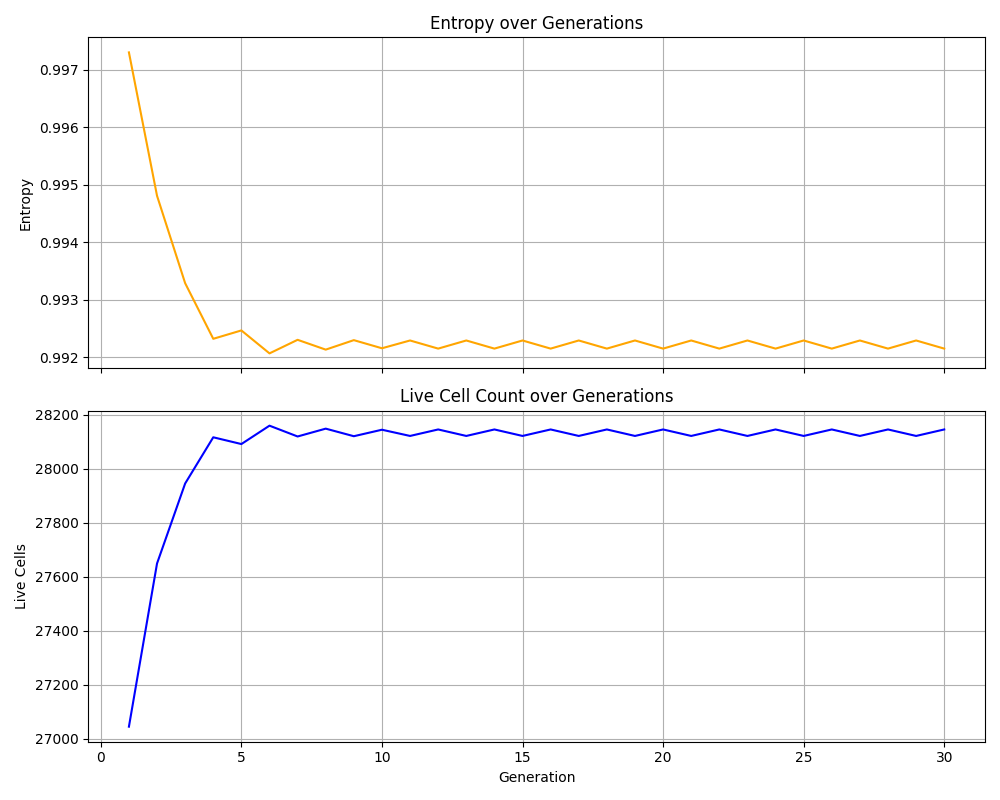
\includegraphics[scale=0.6]{../figures/Figure_3.png}

We once again start from a random state for the grid. The entropy however drops very quickly, flattens and stays consistent. The grid enters a stable pattern and arrives to this pattern very quickly. The population quickly grows to become a highly stable one, with structures containing long corridors, walls, and voids.

\subsubsection{Improvements \& Next Steps}
The current engine is really good. It can simulate pretty much any rule you throw at it and at a really quick speed too. However, once you start scaling the grid to larger and larger dimensions, the inefficient algorithm I used to "tick" the simulation starts to show its true colors. A double for loop over the grid, checking how each cell should move, then pushing that data to a separate copy of the grid turns out to be a very slow way of simulating cellular automata. I currently have no clue how to actually go about improving my algorithm. Perhaps some obscure data structure might help out, but I will be searching the internet for ways to go about this.

The next thing I want to improve is the UI of the simulation. More specifically, I want to add more options for how to visualize the simulation. The current method of having the terminal show the simulation is cool, but it is not portable. If I wanted to share a simulation with someone, I would need to use a third party screen recording tool to then share. Instead, I was thinking of adding an option to output the simulation to a GIF. To do this, I would need to add a cli argument for number of steps, after which the simulation will stop running.

Another thing I wanted to improve was adding a way to set some preset cells to be alive and dead before starting the simulation. I actually got some start to this (you can see it in the source code) but it became a problem because the cells would either be in the wrong place on the grid, move out of the grid too quickly, or just not be visible at all. Furthermore, it is hard to preset something through a command line. The grid can include thousands of cells and chosing one individual cell is practically not a viable way to do this.

There is another library in the Rust ecosystem that provides functions to create your own GIF's from rules you provide, and I believe it takes in presets in as well, so I might have to steal some code from them. In fact, midway through my project, I got so stuck I almost decided to scrap everything I had and just rely on using it to finish this project. I'm very glad I didn't however because I feel like I managed to learn a lot from implementing it myself. Plus, I now have an excuse to write more Rust code!


\section{Conclusion}

This project began as a simple curiosity-driven attempt to simulate cellular automata, but it quickly evolved into a deep and rewarding exploration of emergent systems, Rust programming, and simulation design. Through implementing Conway's Game of Life and experimenting with alternative rule sets like Diamoeba and Maze, I gained a firsthand understanding of how simple rules can give rise to remarkably complex and diverse behaviors. The process of writing this engine from scratch, even with its inefficiencies, taught me a great deal about structuring code for extensibility, working with terminal-based interfaces, and collecting and analyzing simulation data.

What started as an idea sparked by a class lecture and a fascinating video about Turing completeness grew into a robust simulation engine capable of visualizing and analyzing a variety of automaton behaviors. The integration with Python for plotting, the CLI-based control via Clap, and the terminal rendering through Ratatui collectively made this not only a functional system, but also a highly educational one.

While there's still much room for improvement—especially in terms of performance optimization, visualization, and initial state configuration—this project laid a solid foundation for future work. I now feel more equipped to take on larger systems-level problems, and I'm excited to explore possible extensions, such as GIF export support and smarter initialization methods. Most importantly, this project reaffirmed the value of building things from the ground up. Even when third-party tools exist, implementing core functionality myself led to a deeper appreciation of the system and significantly improved my understanding of both Rust and simulation design.

This was more than just a programming assignment—it was a chance to create, explore, and grow as a developer and thinker.

\newpage
\section{References}
\nocite{hugcis_rustca}
\printbibliography[heading=none]
\end{document}
